


\begin{frame}{Underwater 3D-Laserscanner}

%\vspace{1em}
\justifying

To explore the concept of {\bf underwater, laser line 3D scanning} we built a 
prototype system. In particular, we were interested in improving the precision
of the scanner by designing a calibration procedure that is simple enough to
be applicable in practise.
\vspace{1.5em}

\twocol{0.5}{
\justifying
In~\cite{Hildebrandt2008a} we suggest to use a planar calibration object that
is fitted with a checkerboard pattern for calibration of the camera and a high
contrast region for detecting the laser line.

\vspace{1.5em}
Our results indicate that this is a feasable approach that could be used in 
non-laboratory environments without too much effort.

}{0.41}{
\vspace{-1.75em}
\begin{figure}
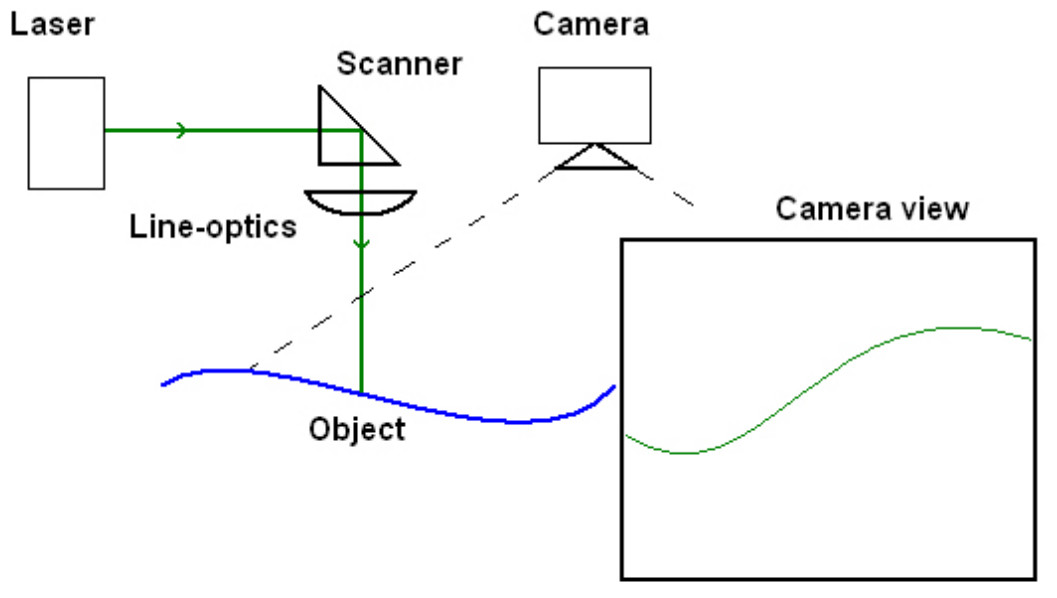
\includegraphics[width=\linewidth]{laser/laser.jpg}

\vspace{-1em}
\caption{\scriptsize Schematic representation of a laser line 3D scanner~\cite{Hildebrandt2008a}.}
\end{figure}
}

\vspace{1.5em}

The concept was followed up on by a number of later projects and led to a 
{\bf spin-off company} (\lnk{https://krakenrobotik.de/}{Kraken Robotik}) founded
by some of my former colleagues.

\begin{center}
\rule{2cm}{0.4pt}\\[0.5em]
\end{center}

\fc{Hildebrandt2008a}{publications/2008-04/2008-04}

\end{frame}
